\begin{figure*}
\centering

\begin{subfigure}[b]{1\textwidth}
       \centering
        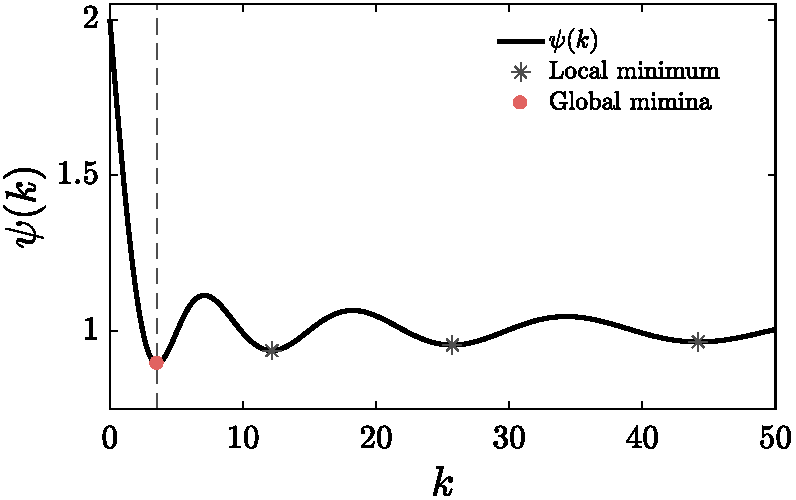
\includegraphics[width=0.333\textwidth]{../ch3/figures/T1_1_PSI}%
        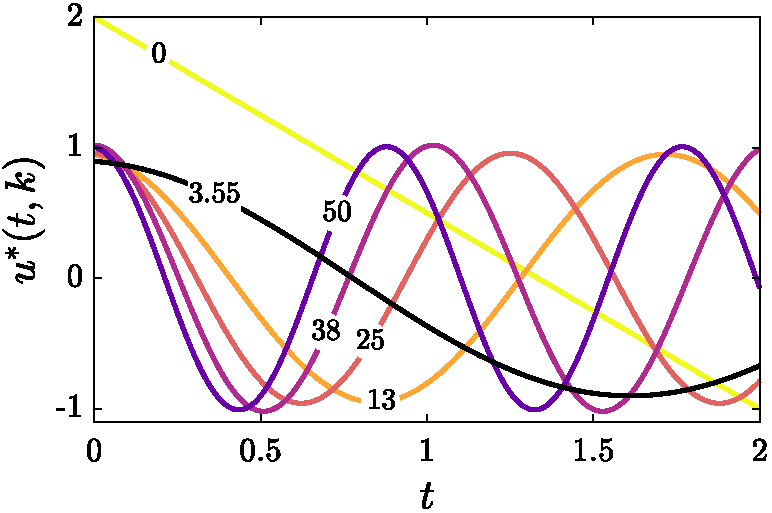
\includegraphics[width=0.333\textwidth]{../ch3/figures/T1_1_U}%
        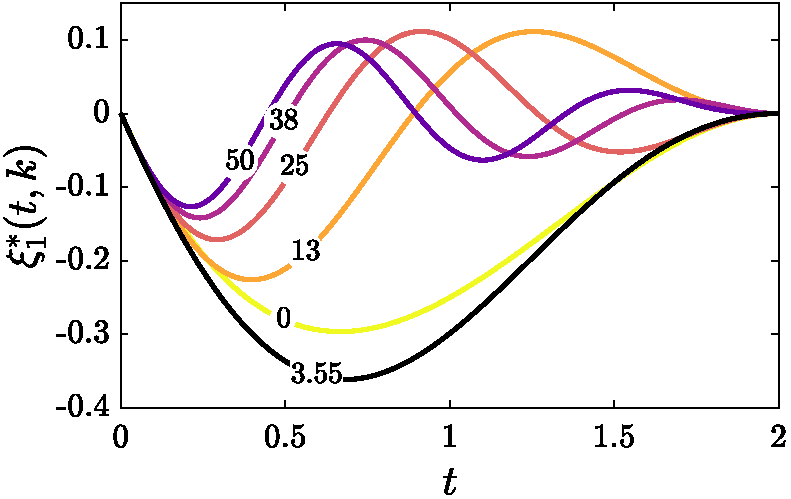
\includegraphics[width=0.333\textwidth]{../ch3/figures/T1_1_X}%
        \caption{TP2 results demonstrating a large number of
local solutions with $t_f = 2$, $x_0 = 0$, and $v_0 = -1$ (different values of $k$ marked).\label{fig:ch3:T1_1}}
\end{subfigure}%

\begin{subfigure}[b]{1\textwidth}
  \centering
  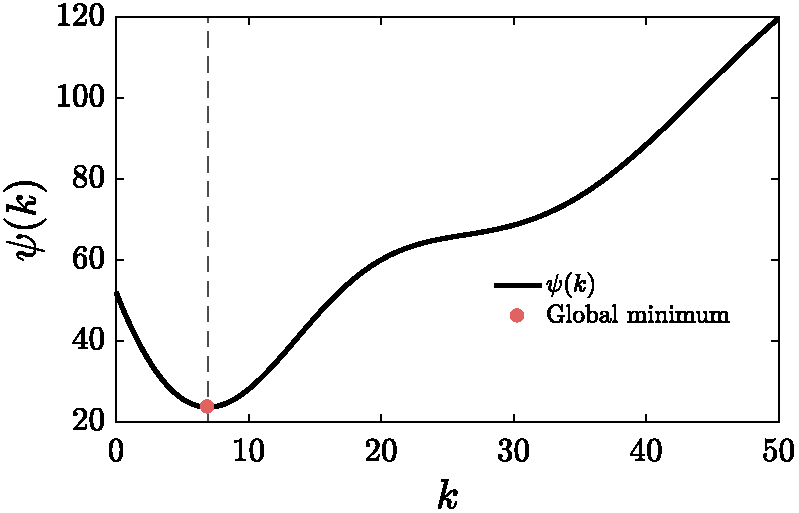
\includegraphics[width=0.333\textwidth]{../ch3/figures/T1_2_PSI}%
  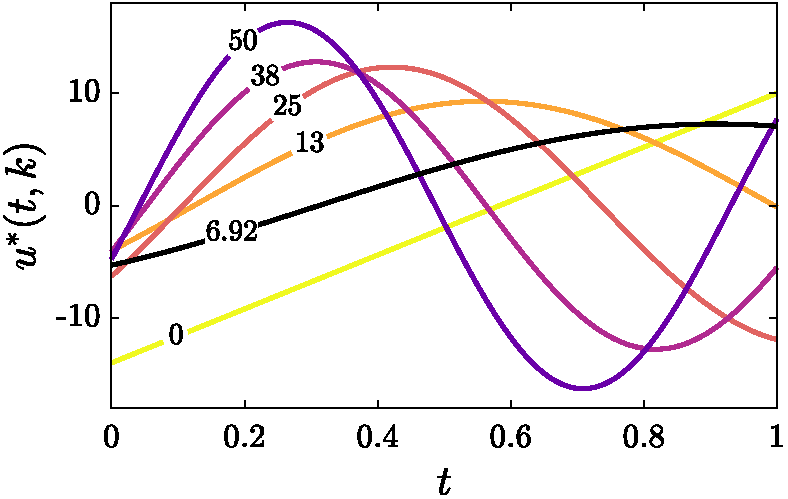
\includegraphics[width=0.333\textwidth]{../ch3/figures/T1_2_U}%
  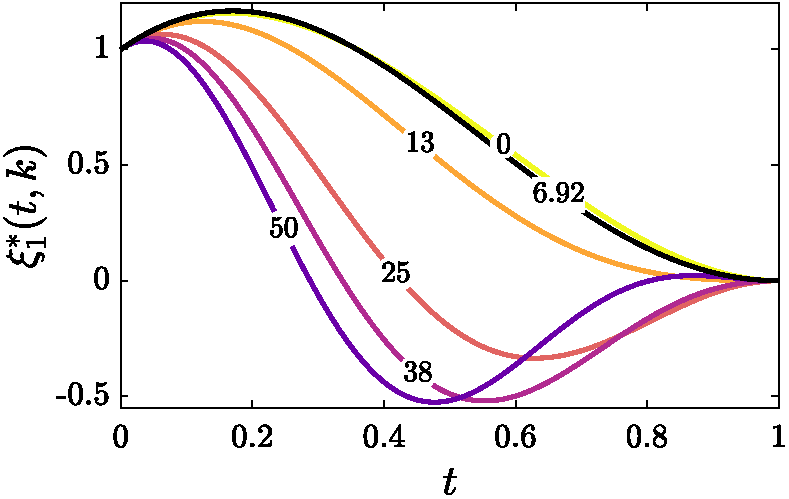
\includegraphics[width=0.333\textwidth]{../ch3/figures/T1_2_X}%
  \caption{TP2 results demonstrating single global minimum with $t_f = 1$, $x_0 = 1$, and $v_0 = 2$ (different values of $k$ marked).\label{fig:ch3:T1_2}}
\end{subfigure}%

\begin{subfigure}[b]{1\textwidth}
  \centering
  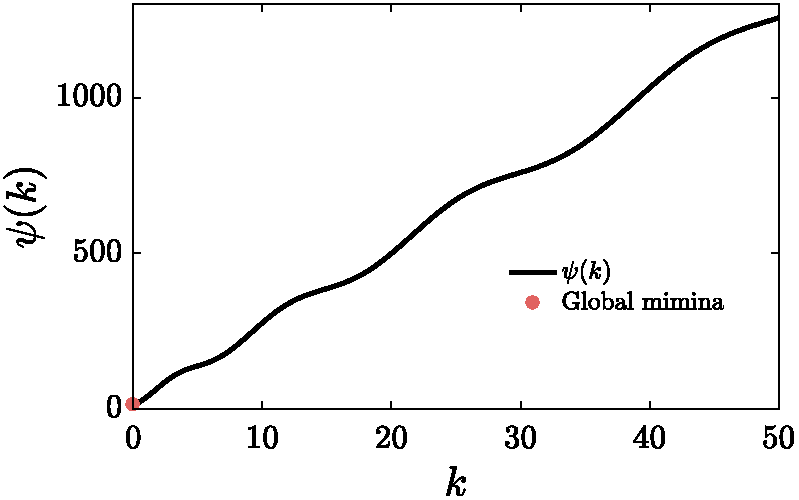
\includegraphics[width=0.333\textwidth]{../ch3/figures/T1_3_PSI}%
  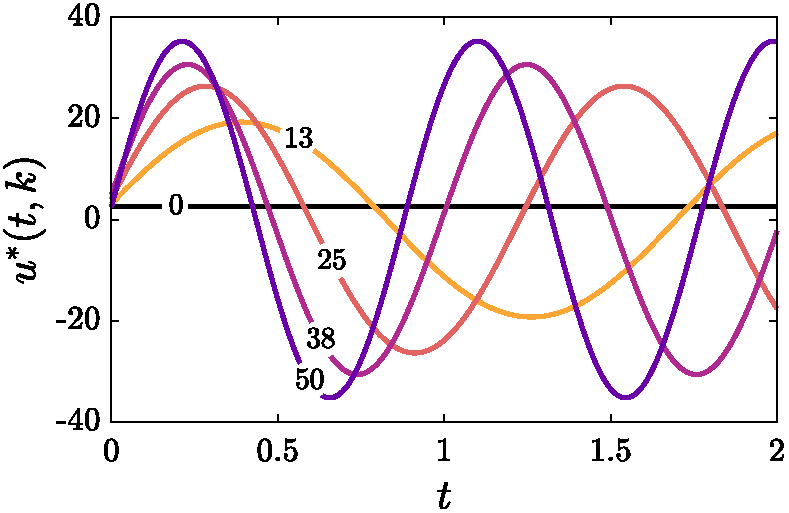
\includegraphics[width=0.333\textwidth]{../ch3/figures/T1_3_U}%
  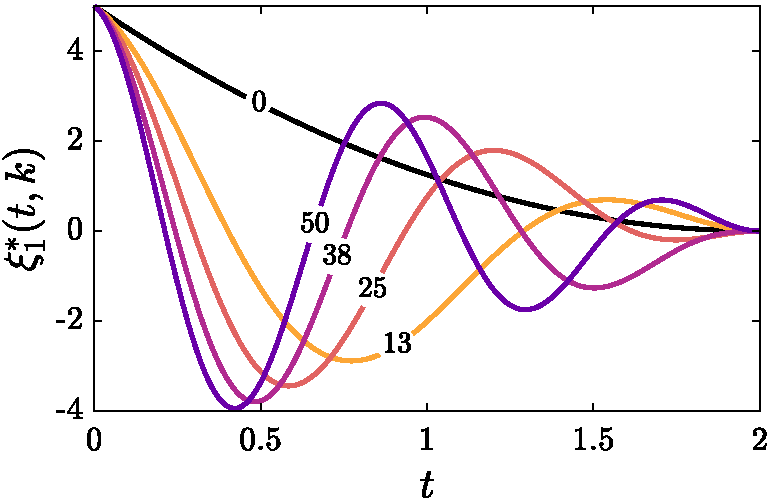
\includegraphics[width=0.333\textwidth]{../ch3/figures/T1_3_X}%
  \caption{TP2 results demonstrating degenerate plant solution with $t_f = 2$, $x_0 = 5$, and $v_0 = -5$ (different values of $k$ marked).\label{fig:ch3:T1_3}}
\end{subfigure}%

\caption[Co-design transfer problem (TP2) results]{Co-design transfer problem (TP2) results for various values of the problem parameters.\label{fig:ch3:T1}}
\end{figure*}% 